% OK !
\section{Analyse du marché et des besoins, élaboration du cahier des charges}
Afin de développer un produit qui puisse convenir aux besoins des personnes souffrant de bégaiement ainsi qu'aux orthophonistes, j'ai effectué des recherches pour définir les exercices utilisés par les orthophonistes lors des séances avec leurs patients. Le projet devant être réalisé en seulement 12 semaines, j'ai décidé de concentrer mes recherches uniquement en ligne sans démarcher de réels orthophonistes, ce qui m'aurait permis de cerner plus précisément les besoins, mais qui m'aurait aussi pris beaucoup plus de temps.

J'ai également réalisé une étude comparative des applications actuellement disponible sur le marché Android, le tableau récapitulatif de cette étude est disponible en annexe \ref{appendix:market}. Cette étude a révélé un manque d'application complète comprenant différents types d'exercices. Les applications actuellement disponibles se concentrent souvent sur un seul exercice. Par ailleurs, aucune application propose de faire le lien entre les bègues et leurs orthophonistes.

Afin de décrire complètement le but de l'application, le contexte d'utilisation dans lequel elle s'inscrit (\textit{Par qui ? Comment ? Pourquoi ?}), ses fonctionnalités et les exigences non-fonctionnelles (sécurité, maintenabilité, \textit{scalability}, etc.), j'ai rédigé un \textit{Software Requirements Specification (SRS)}. Un \textit{SRS} est un document qui fournit une description complète de la façon dont le produit est censé fonctionner, en particulier ce document décrit les interactions de l'utilisateur sur le produit et les éventuelles contraintes et exigences non-fonctionnelles à respecter (lois et régulations, protocoles à utiliser, limitations matérielles, sécurité, etc.). La table des matières de ce document est disponible dans l'annexe \ref{appendix:srs}. Ce document décrit précisement les interactions de l'utilisateur récapitulées dans le diagramme de cas d'utilisation de la figure \ref{fig:srs}. Voir l'annexe \ref{appendix:srs_example} pour un exemple de spécification d'un cas d'utilisation.

\begin{figure}[h]
  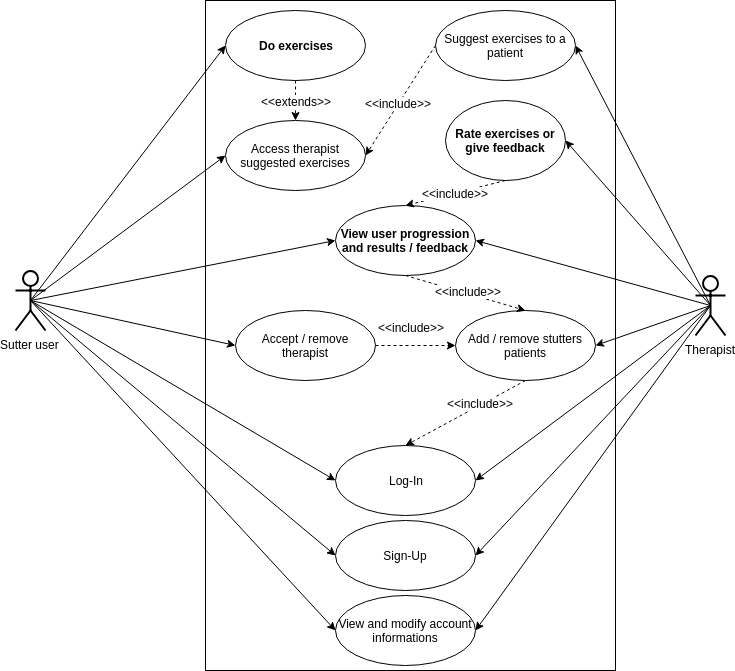
\includegraphics[width=.9\linewidth]{content/imgs/usecase.png}
  \caption{Diagramme cas d'utilisation}
  \label{fig:srs}
\end{figure}

\subsection{Résumé de cahier des charges de l'application}
\label{sec:resume_cdc}

L'application est destinée à être utilisée par des personnes souffrant de bégaiement et par des orthophonistes. Lors du premier démarrage de l'application, l'utilisateur devra alors choisir s'il souhaite utiliser l'application en tant que bègue ou en tant qu'orthophoniste.

\subsubsection{Utilisateurs bègues}

Les bègues auront à disposition une liste d'exercices pour s'entraîner à mieux contrôler leurs flux de paroles. Chaque exercice sera paramétrable pour convenir aux besoins de l'utilisateur. En particulier, les exercices pourront utiliser des ressources que l'utilisateur devra lire à voix haute. Ces ressources devront être récupérées via une collection de ressources partagée possédant plusieurs types de ressources : des mots, des phrases et des textes. Le bègue pourra alors choisir sur quel type de ressource il souhaite s'entraîner. Les exercices pourront aussi s'appuyer sur d'autres éléments, par exemple un enregistreur vocale ou vidéo afin d'enregistrer l'exercice. L'utilisateur pourra choisir d'activer ou non ces enregistreurs. Voici quatre exercices types rentrant dans le cadre de l'application :

\begin{itemize}
  \item \textbf{Metronome} : le bègue s'entraîne à parler avec un rythme régulier grâce à un métronome (appareil émettant un signal -- visuel et/ou sonore -- à intervalle de temps régulier) ;
  \item \textbf{Reading} : le bègue parle librement sur des ressources de son choix (mot, texte, phrase) ;
  \item \textbf{Delayed Auditory Feedback (DAF)} : le bègue parle puis entend le retour de sa voix quelques dizaines de millisecondes après ;
  \item \textbf{Mirroring} : le bègue s'entraine à parler avec un retour vidéo de sa tête pour analyser ses mouvements faciales.
\end{itemize}

L'utilisateur bègue pourra accéder à sa progression. La progression est constituée de l'historique de tous les exercices effectués. Ces exercices contiendront l'éventuel enregistrement vocal ou vidéo, les ressources utilisées lors de l'exercice ainsi qu'un commentaire de son éventuel orthophoniste (voir ci-après). La progression de l'utilisateur devra aussi pouvoir être visualisée graphiquement grâce à une courbe illustrant le pourcentage de réussite de prononciation des mots prononcés lors des exercices.

L'utilisateur bègue pourra décider de synchroniser ses exercices dans le \textit{cloud}. Pour ce faire, il devra se créer un compte avec un nom, une adresse mail et un mot de passe. Une fois un exercice synchronisé dans le \textit{cloud}, il sera accessible par son éventuel orthophoniste qui pourra alors ajouter un commentaire sur cet exercice. Les utilisateurs bègues peuvent donc ajouter un orthophoniste autorisé à avoir accès à tous leurs exercices synchronisés. Pour ajouter un orthophoniste, ils devront connaître son identifiant personnel (voir ci-après). Ils pourront bien entendu révoquer l'accès de cet orthophoniste aux exercices à tout moment.

\subsubsection{Utilisateurs orthophonistes}

Pour utiliser les fonctionnalités de l'application, les orthophonistes devront créer un compte (comme pour les bègues, avec un nom d'utilisateur, un courriel et un mot de passe). Une fois le compte créé, l'orthophoniste aura accès à son identifiant personnel ainsi que la liste de tous les utilisateurs bègues l'ayant ajouté comme orthophoniste. Un tel utilisateur est alors le \textit{patient} de l'orthophoniste. L'orthophoniste pourra visualiser la progression de ses patients. Il pourra aussi supprimer des patients de sa liste.















% eof
